\chapter{Семантическая теория программ для ostis-систем}
\chapauthortoc{Зотов Н.В.\\Шункевич Д.В.}
\label{chapter_programs}

\vspace{-7\baselineskip}

\begin{SCn}
\begin{scnrelfromlist}{автор}
	\scnitem{Зотов Н.В.}
	\scnitem{Шункевич Д.В.}
\end{scnrelfromlist}

\bigskip

\scntext{аннотация}{Несмотря на активное развитие и использование языков программирования, общей теории программ, на основе которой можно было бы проектировать и разрабатывать прикладные системы, на данный момент не существует. В данной главе предлагается семантическая теория программ для ostis-систем. Глава показывает особенности представления и ключевые моменты процесса интерпретации программ в ostis-системах.}

\bigskip

\begin{scnrelfromlist}{подраздел}
	\scnitem{\ref{sec_programs_problems_and_tasks}~\nameref{sec_programs_problems_and_tasks}}
	\scnitem{\ref{sec_programs_ontologies}~\nameref{sec_programs_ontologies}}
	\scnitem{\ref{sec_programs_solution}~\nameref{sec_programs_solution}}
	\scnitem{\ref{sec_programs_method_syntax_and_semantic}~\nameref{sec_programs_method_syntax_and_semantic}}
	\scnitem{\ref{sec_programs_method_representation_language_syntax_and_semantic}~\nameref{sec_programs_method_representation_language_syntax_and_semantic}}
	\scnitem{\ref{sec_programs_help_system}~\nameref{sec_programs_help_system}}
	\scnitem{\ref{sec_programs_method_kriteria}~\nameref{sec_programs_method_kriteria}}
\end{scnrelfromlist}

\bigskip

\begin{scnrelfromlist}{ключевое понятие}
	\scnitem{метод}
	\begin{scnindent}
		\scnitem{программа}
	\end{scnindent}
	\scnitem{язык представления методов}
	\begin{scnindent}
		\scnitem{язык программирования}
	\end{scnindent}
	\scnitem{синтаксис языка представления методов}
	\scnitem{денотационная семантика языка представления методов}
	\scnitem{операционная семантика языка представления методов}
	\scnitem{эффективность метода}
\end{scnrelfromlist}

\begin{scnrelfromlist}{ключевой знак}
	\scnitem{Семантическая теория программ для ostis-систем}
\end{scnrelfromlist}

\bigskip

\begin{scnrelfromlist}{библиографическая ссылка}
	\scnitem{***}
\end{scnrelfromlist}

\end{SCn}

\section*{Введение в Главу \ref{chapter_programs}~\nameref{chapter_programs}}

За долгий период развития компьютерных систем практически сняты аппаратные ограничения на решение различных задач. Оставшиеся ограничения отводятся на долю программного обеспечения. Прежде всего эти ограничения связаны с текущими проблемами развития программного обеспечения:
\begin{textitemize}
    \item \myuline{аппаратная сложность опережает} умение человечества строить \myuline{программные компьютерные системы}, использующее потенциальные возможности аппаратуры;
    \item навыки и \myuline{технологии} разработки программ \myuline{отстают от требований}, предъявляемых к разработке программ нового поколения;
    \item возможностям эксплуатировать существующие программы угрожает \myuline{низкое качество их разработки}.
\end{textitemize}

Ключом к решению этих проблем является глубокое понимание и грамотное использование существующих языков программирования как основного инструмента для массового создания программных компьютерных систем нового поколения.

В данной главе акцент делается на достижение следующих результатов:
\begin{textitemize}
    \item (1) изложить классические основы, отражающие накопленный мировой опыт в области разработки и применения современных языков программирования;
    \item и (2) систематизировать основные результаты в этой области и представить их в виде единой унифицированной семантической теории программ.
\end{textitemize}

В данной главе подробно описываются проблемы текущего состояния в области программ и языков программирования. Она посвящена базовым понятиям теории языков программирования, дается обзорная характеристика областей применения языков программирования, достаточно востребованных современным человеческим обществом, рассматриваются способы представления и интерпретации программ различных языков программирования, подробно описываются формы и содержание критериев для оценки эффективности языков.

\section{Проблемы текущего состояния в области разработки и применения языков программирования}
\label{sec_programs_problems_and_tasks}

В современную эру развития информационных технологий существует огромное количество языков программирования, каждый из которых имеет своё важное назначение в области проектирования программных систем. Каждый язык демонстрирует не только свою специфику, но имеет свои достоинства и недостатки. Многообразие \textit{языков программирования} \cite{Sebesta2012} и решений, созданных на них, настолько велико, что очень легко потеряться в море информации о всех аспектах применения и проектирования языков программирования. Кроме этого, основная проблема заключается не в количестве существующих решений в области разработки и применения современных \textit{языков программирования}, а количестве форм (!), на которых представляются конкретные \textit{языки программирования}. Так, декларативные знания, то есть знания, являющиеся, например, спецификацией какой-то программы, и процедурные знания, то есть знания, которые являются программами, принадлежащими какому-то языку программирования, представляются совершенно различными способами, методами и средствами.

В связи со сказанным можно выделить следующие ключевые проблемы в области разработки и применения современных языков программирования:
\begin{textitemize}
    \item Поскольку количество языков программирования растёт с увеличением потребности в них, то растут и потребности в описании этих языков программирования для дальнейшего использования и проектирования прикладных систем. Это в свою очередь требует высокого уровня качества спецификации конкретного языка: и описания синтаксиса и семантики конструкций этого языка, и описания средств и методов реновации инструментальных средств, обеспечивающих интерпретацию или трансляцию этого языка. То есть, с увеличением количества языков программирования растёт не только многообразие форм представления знаний (языков программирования), но и количество программных систем на различных формах представления знаний \scncite{Zapata2010}.
    \item Большое многообразие форм представления знаний, как говорилось выше, предоставляет большой спектр возможностей проектирования программных компьютерных систем на каждой из них. Получается, чтобы произвести интеграцию нескольких программных систем, реализованных на разных языках программирования, необходимо сделать так, чтобы системы могли коммуницировать между собой на каждом их тех языков, на котором они реализованы \scncite{Golenkov2019a}. Так, стремление к использованию существующих программных компонентов затрудняется реализацией самих компонентов, поскольку чтобы объединить эти компоненты необходимо изменить их программный код \cite{Penta2020}, \cite{Scalabrino2016}. Наличие многообразие форм затрудняет реализацию совместимых интероперабельных программных компьютерных систем \scncite{Golenkov2012}.
    \item С ростом сложности программного кода, уменьшается количество способных понять его смысл. Современные разработчики создают программные компьютерные системы, не учитывая полный её жизненный цикл \cite{Brooks2021}. Системы должны постоянно обновляться и совершенствоваться с развитием технологий, на которых она основана \cite{Sellitto2022}. Это должно обеспечиваться хорошей документацией реализации компонентов этих систем -- это снижает не только потребности в привлечении новых ресурсов и кадров, но и способствует снижению реинжиниринга программных компьютерных систем \cite{Penta2020}, \cite{Scalabrino2016}.
    \item Полная автоматизация проектирования программных компьютерных систем невозможна, поскольку современные языки, на которых они проектируются не имеют свойства рефлексивности -- системы не могут познавать и понимать себя и развиваться почти в полной мере самостоятельно. Таким образом, существующие компьютерные системы не являются как таковыми интеллектуальными, потому что не имеют необходимых им свойств \scncite{Golenkov2022a}.
    \item Ключом к легкому и глубокому освоению конкретного языка как основного профессионального инструмента программиста является понимание общих принципов построения и применения языков программирования \cite{Turner2007}, \cite{Constanta2022}, описываемых их общей теорией. До сегодняшнего дня, общей теории языков программирования до сих пор не существует, что затрудняет разработку, верификацию и использование новых и существующих языков программирования. Без общей теории языков программирования каждый может разрабатывать принципиально общие методы и средства так, как хочется, а не так, как требуется \scncite{Golenkov2012}.
    \item Достижение максимума услуг и средств при минимуме затрат возможно только путём глубокого понимания принципов построения языков программирования за счёт простоты средств и методов представления знаний. Сложное нужно сводить к простому и изъяснять простыми понятиями, не создавая дополнительной иллюзии важности \cite{Sellitto2022}, \cite{Chaparro2014}, \cite{Posnett2011}.
\end{textitemize}

Все эти проблемы связаны и являются проблемами текущего состояния направлений развития в области Искусственного интеллекта \cite{Skeeter2020}, \cite{Constanta2022}.

Итак, для решения перечисленных проблем необходимо создавать комфортные условия для реализации компьютерных систем, семантически совместимых и интероперабельных между собой. В контексте языков программирования необходима общая \textit{Семантическая теория программ для интеллектуальных компьютерных систем нового поколения}, которая:
\begin{textitemize}
    \item \myuline{позволит} без больших усилий и затрат \myuline{интегрировать имеющиеся решения} в области проектирования программ компьютерных систем \scncite{Golenkov2019};
    \item \myuline{объединит формы представления знаний} декларативного и процедурного вида;
    \item \myuline{будет иметь широкий спектр средств} не только для описания синтаксиса и семантики существующих языков программирования, но и для проектирования новых аналогов;
    \item \myuline{будет понятна} не только человеку, но и машине \scncite{Zapata2010};
    \item \myuline{обозначит принципы}, по которым необходимо проектировать \textit{языки программирования нового поколения}.
\end{textitemize}

К проектированию таких общих теорий, строго говоря, нужно подходить с высокой степенью важности. Проектируемые \textit{компьютерные системы} должны всегда иметь возможности использовать те свойства, которые им начертаны. Для того, чтобы и эта теория могла быть использована как некоторая система знаний о том, как надо проектировать и использовать языки программирования и программы в \textit{программных компьютерных системах}, и том, как интерпретировать их программы, необходимо, чтобы эта теория была описана средствами и методами, которыми проектируются эти \textit{программные компьютерные системы}. Речь идёт о том, что принципиально важным подходом к проектированию общей теории программ является онтологический подход \scncite{Zapata2010}, \scncite{Golenkov2019}, \cite{Sales2022}, \cite{Samaa2020}.

Для воплощения данных идей необходимо изучить и интегрировать опыт, накопленный в области разработки и применения современных языков программирования. Поэтому далее будут рассмотрены результаты других исследований в области проектирования общей теории языков программирования и программ.

\section{Существующие онтологии языков программирования}
\label{sec_programs_ontologies}

В большинстве, идеи, предлагаемые в научных работах по исследованию языков программирования, безусловно являются востребованными и полезными для проектирования \textit{программных компьютерных систем}. Так, идея о том, что языки программирования и программы, реализуемых на них, должны быть организованы в общую таксономию понятий, является основополагающей, поскольку обеспечивает наиболее качественную среду для проектирования и реализации \textit{программных компьютерных систем}. Общая теория программ нужна не только для того чтобы описывать термины и понятия как некоторую спецификацию, используемую для проектирования \textit{программных компьютерных систем} (что тоже не мало важно), но и для того, чтобы определять качество языков программирования и программ по таким вопросам, как: \scnqq{Является ли данный язык языком программирования}, \scnqq{Является ли данное знание программой}, \scnqq{Насколько эффективна данная программа}, \scnqq{Какова степень интеллекта данной программной системы} и т. д. Данные идеи предложены и рассмотрены в работах Raymond Turner \cite{Eden2007}, \cite{Turner2012}.

До сегодняшнего дня существует большое количество аналогов онтологий языков программирования и программ. Примеры можно найти в работах \cite{Lando2007}, \cite{Lando2009}, \cite{Turner2007}.  Также стоит отметить разработанные онтологии программ \cite{Turner2012}, \cite{Turner2014}, \cite{Jacobs2022}, система понятий в которых определяется строго и однозначно на формальных языках: языках логики и языках описания грамматик формальных языков. Однако ни одна из них не является таким результатом, который можно было бы использовать при проектировании \textit{программных компьютерных систем} без существенных проблем. Разработанные онтологии сосредотачивают в себе лишь краткое описание связанных между собой понятий, но общей картины того, как данные онтологии можно использовать в конкретных задачах, почти не видно.

Сегодня встречаются и вовсе протовоположные суждения о назначении программ и языков программирования \cite{Rapaport2020}, противоречащие формальным основам Искусственного интеллекта \cite{Grimmelmann2022}. \textit{Программные компьютерные системы} должны быть не только понятны человеку, но и сами должны понимать себя, свои возможности, намерения, действия и цели, и понимать себе подобные кибернетические системы. Только таким образом человечество и результаты его деятельности в виде каких-то конкретных систем смогут работать сообща, дополняя друг друга и преумножая свои результаты \scncite{Golenkov2012}.

В результате анализа приведенных работ можно сделать вывод о том, что:
\begin{textitemize}
    \item общей теории программ и языков программирования, которая могла быть задействована при решении любой прикладной задачи и представлении и реализации средств проектирования компьютерных систем до сих пор не сложилась;
    \item унификация представления средств описания и реализации по этим описании как главный аргумент к оперированию смысловому представлению знаний, к полному взаимопониманию между компьютерными системы вовсе не рассматривается;
    \item программы и совокупности этих программ в виде программных компьютерных систем реализуются в большинстве случаев в индивидуальном порядке и плохо документируются, что усложняет их использование, интеграцию с другими программами и программными компьютерными система, тестирование и совершенствование.
\end{textitemize}

Ключом к решению всех этих проблем является общая \textit{Технология проектирования компьютерных систем нового поколения}, на базе которой можно построить общую теорию программ (дисциплину программирования) \cite{Deikstra1978}, которая будет рассмотрена дальше.

\section{Предлагаемый подход к разработке технологий программирования для ostis-систем}
\label{sec_programs_solution}

Поскольку количество \textit{языков программирования} растёт с увеличением потребности в них, то растут и потребности в описании этих \textit{языков программирования} для проектирования и разработки \textit{программных компьютерных систем} на этих языках. То есть, с увеличением количества \textit{языков программирования} растёт не только многообразие форм представления знаний, но и количество \textit{программных компьютерных систем} на различных формах представления знаний. Это в свою очередь требует не только качественной спецификации конкретного \textit{языка программирования} для разработки \textit{программ} на этом языке, но и новых требований к существующим разработчикам. В итоге, это влечёт за собой появление барьеров и для создания семантически совместимых и интероперабельных программных компьютерных систем, и для обеспечения благоприятной среды для взаимодействия их разработчиков.

Для преодоления данных проблем нет необходимости пересматривать уже существующие решения в области разработки программного обеспечения. Необходимо создавать принципиально новые языки программирования, а также программных компьютерных систем на них, в которых будут учтены и решены существующие проблемы. Для этого следует учитывать следующие принципы программирования этих систем:
\begin{itemize}
	\item Расширение многообразия форм представления знаний происходит за счёт появлений новых синтаксических конструкцих в \textit{языках программирования}. Поэтому разработка \textit{языков программирования} должна сводиться к уточнению \textit{синтаксиса} и \textit{семантики} уже существующих \textit{языков программирования}. При этом все \textit{языки программирования} должны являться подъязыками некоторого базового \textit{языка программирования}.
	\item Нет необходимости в создании дополнительных языков, с помощью которых можно описывать семантику программ на \textit{языках программирования}. Наоборот, \textit{языки программирования}, на котором разрабатываются программы, должен позволять своими же средствами описывать \textit{семантику} \textit{программ} на этом же языке.
	\item Документирование \textit{программ}, в том числе \textit{программных компьютерных систем}, должно минимизироваться за счёт этапов их качественного проектирования и разработки. Смысл конструкций \textit{программ} \textit{языков программирования} должен быть настолько ясным и понятным, чтобы использование программ на этом \textit{языке программирования} не требовало дополнительных ресурсов и инструментов как и у разработчиков этих программ и систем, таких и у новых разработчиков.
	\item Появление новых программ должно влечь за собой к расширению \textit{Библиотеки многократно используемых программ} и к уменьшению количества семантически эквивалетных программ. Таким образом, программы должны быть не только максимально образом совместимыми между собой, но открытыми для переиспользования в других \textit{программных компьютерных системах нового поколения}.
	\item Полный жизненный цикл разработки новых программ должен обеспечиваться теми же средствами и \textit{языками программирования}, на которых разрабатываются эти программы.
	\item Сложность программ и \textit{программных компьютерных систем} должна сводиться к минимуму. То, что выглядит сложно, должно и может быть сделано максимальное проще. 
	\item Построение качественного коллектива \textit{программных компьютерных систем} может быть обеспечено только совместимостью и интероперабельностью самих систем, и коллективов тех разработчиков, которые их создают.
\end{itemize}

Несмотря на обширное разнообразие используемых человечеством классических технологий, общего решения, позволяющего решить поставленные проблемы в комплексе, не существует. Накопленный опыт в сфере проектирования и реализации компьютерных систем показывает, что для более качественной и эффективной реализации различных методов существующие технологии не приспособлены для решения комплексных задач. Для повышения качества разработки сложных систем необходимо разрабатывать и использовать принципиально новые технологии программирования.

Почему \textit{Технология OSTIS} является ключом к решению описанных проблем в области проектирования и применения языков программирования?
\begin{textitemize}
    \item {Стандарт Технологии OSTIS \cite{Standard2021} уже реализует базовые средства, необходимые для проектирования и разработки интероперабельных \textit{программных компьютерных систем}, в основе которых лежит смысловое представление знаний. Это устраняет не только необходимость создания онтологий верхнего уровня, которые должны быть использованы в общей теории программ как базовые для описания понятий этой теории, но и помогает проектировать решения согласованно с другими онтологиями. В результате формируется общая слаженная картина мира, которая (1) непротиворечива, то есть согласована, (2) однозначно трактуема, (3) универсальная и, (4) самое главное, понятна для каждого.}
    \item {Технология OSTIS проектируется одним языком унифицированного представления знаний, называемым SC-кодом. Смысл программ и \textit{языков программирования} понятен и однозначен тогда и только тогда, когда этот смысл описывается на одном общем языке, понятному любой кибернетической системе.}
    \item {SC-код синтаксически минимален. Для описания объектов и связей между ними используется минимальное количество знаков. В то же время многообразие этих связей сводится к многобразию знаковых конструкций. Всё это обеспечивается за счёт представления информации в виде графовых структур \cite{Kasyanov2003}, \cite{Petrov1978}.}
    \item {SC-код не просто удобен для описания и проектирования каких-то сложных объектов -- с его помощью можно проектировать и реализовывать любые \textit{языки представления знаний}, в том числе программ, компьютерные системы и, вообще, описывать реальный мир.}
    \item {Онтологический и компонентный подходы \cite{Sales2022}, \cite{Samaa2020} к проектированию любых сложных объектов обеспечивают выполнение главных принципов, по которым должны проектироваться современные системы. То, что реализовано и можно использовать, нужно переиспользовать везде \cite{O4IS2007}, \cite{Molorodov2019}.}
\end{textitemize}

Проектирование и реализация программы на каком-либо \textit{языке программирования} должна сводиться к описанию её \textit{синтаксиса} и \textit{денотационной семантики} в базе знаний ostis-системы с помощью некоторой библиотеки предметных областей и онтологий программ, описываемой в рамках этой базы знаний. Для этого нужна онтология программ, которые позволили бы в достаточном объёме описывать программы на любых языках программирования в ostis-системах. Такой подход позволяет не только описывать сложноструктурированные объекты простым и понятным языком, но и позволяет унифицировать представление различных видов знаний. Тем самым, информация о программах и сами программы представляются на одном и том же языке (имеют один синтаксис), но содержательно описываются при помощи разных онтологий. Таким образом, \uline{решением всех проблем будет являться общая теория программ}, однозначно соответствующей некоторой онтологии программ, c помощью которых можно было б описывать синтаксис и денотационную семантику любых программ в ostis-системах.

Таким образом, результатом данной главы является \textit{Предметная область и онтология программ} (далее - Предметная область и онтология методов), с помощью которой можно описывать синтаксис, денотационную и операционную семантику различных методов в ostis-системах. \textit{Предметная область и онтология методов} является дочерней предметной областью по отношению к \textit{Предметной области и онтологии информационных конструкций и языков}. Это означает, что она наследует все свойства исследуемых в ней понятий и отношений.

\begin{SCn}
\scnheader{Предметная область и онтология информационных конструкций и языков}
\begin{scnrelfromlist}{дочерняя предметная область}
    \scnitem{Предметная область и онтология языков}
    \begin{scnindent}
        \begin{scnrelfromlist}{дочерняя предметная область}
            \scnitem{Предметная область и онтология естественных языков}
            \scnitem{Предметная область и онтология формальных языков}
        \end{scnrelfromlist}
    \end{scnindent}
\end{scnrelfromlist}
\end{SCn}

\begin{SCn}
\scnheader{Предметная область и онтология формальных языков}
\begin{scnrelfromlist}{дочерняя предметная область}
    \scnitem{Предметная область и онтология языков представления знаний}
    \begin{scnindent}
        \begin{scnrelfromlist}{дочерняя предметная область}
            \scnitem{\scnkeyword{Предметная область и онтология методов}}
        \end{scnrelfromlist}
    \end{scnindent}
\end{scnrelfromlist}
\end{SCn}

\begin{SCn}
\scnheader{Предметная область и онтология методов}
\begin{scnrelfromlist}{дочерняя предметная область}
    \scnitem{Предметная область и онтология методов ostis-систем}
    \begin{scnindent}
        \begin{scnrelfromlist}{дочерняя предметная область}
            \scnitem{Предметная область и онтология процедурных методов ostis-систем}
        \end{scnrelfromlist}
    \end{scnindent}
\end{scnrelfromlist}
%%%% описать классы и отношения
\end{SCn}

Каждая теория должна быть согласована понятийно. Несмотря на то, что в литературе сложилась разное трактование понятия \textit{языка программирования}, должно быть одно универсальное. Для этого вместо языков программирования далее \myuline{будем говорить о языках представления методов}, а вместо программ этих языков программирования -- о методах как знаковых конструкциях языков представления методов. Такое решение обосновывается тем, что обычно язык выступает в роли инструмента какого-то знания определенного вида, а термин \textit{языка программирования} является вырожденным, поскольку стоит говорить не о языках, на которых что-то можно программировать, а о языках, на которых можно представлять знания определённого вида, в данном случае -- знания процедурного типа. Сами термины \scnqqi{языка программирования} и \scnqqi{программы} будем считать неосновными идентификаторами понятий \scnqqi{языка представления методов} и \scnqqi{метода}, соответственно. Также это правило применяется на все понятия, используемые в данной главе и содержащие термин "метод".

Общая \textit{Семантическая теория программ в ostis-системах} не отрицает весь накопленный опыт в сфере разработки современных \textit{технологий программирования}. Наоборот, предлагаемая в данной главе идея позволяет переиспользовать те проверенные инструменты и методы для наиболее быстрой и качественной реализации программ в сложных \textit{программных компьютерных системах}.

\section{Синтаксис и семантика программ в ostis-системах}
\label{sec_programs_method_syntax_and_semantic}

\begin{SCn}
	
\begin{scnrelfromlist}{подраздел}
	\scnitem{\ref{sec_programs_method_syntax}~\nameref{sec_programs_method_syntax}}
	\scnitem{\ref{sec_programs_method_den_semantic}~\nameref{sec_programs_method_den_semantic}}
	\scnitem{\ref{sec_programs_method_op_semantic}~\nameref{sec_programs_method_op_semantic}}
\end{scnrelfromlist}

\bigskip

\begin{scnrelfromlist}{ключевое понятие}
	\scnitem{спецификация метода*}
	\scnitem{денотационная семантика метода*}
	\scnitem{операционная семантика метода*}
\end{scnrelfromlist}

\bigskip

\begin{scnrelfromlist}{библиографическая ссылка}
	\scnitem{***}
\end{scnrelfromlist}
	
\end{SCn}

\textit{Синтаксис} и \textit{семантика} метода представляют его \textit{спецификацию}. Семантику метода можно рассматривать с двух ракурсов: как множество знание, связанных между собой, что определяется \textit{денотационной семантикой} данного \textit{метода}, и как знание, которое может быть интерпретировано другим методом, что определяется операционной семантикой данного метода.

\begin{SCn}
\scnheader{спецификация метода*}
\begin{scnrelfromset}{разбиение}
    \scnitem{синтаксис метода*}
    \scnitem{денотационная семантика метода*}
    \begin{scnindent}
        \scnidtf{обобщенная формулировка класса задач, решаемых с помощью данного метода*}
        \scnrelboth{семантически близкий знак}{обобщенная формулировка задач соответствующего класса методов*}
    \end{scnindent}
    \scnitem{операционная семантика метода*}
    \begin{scnindent}
        \scnidtf{перечень обобщенных агентов, обеспечивающих интерпретацию метода*}
        \scnidtf{семейство методов интерпретации данного метода*}
        \scnidtf{формальное описание интерпретатора заданного метода*}
    \end{scnindent}
\end{scnrelfromset}
\end{SCn}

\subsection{Синтаксис программ в ostis-системах}
\label{sec_programs_method_syntax}

Любый \textit{метод} состоит из \textit{информационных конструкций}, которые задают порядок действий в базе знаний, с помощью которых нужно перейти от исходного состояния к \myuline{целевому}, решив таким образом какую-то конкретную задачу. Так, например, в процедурном методе любой такой оператор представляет собой некоторую математическую функцию. Для композиции этих функций в более крупные фрагменты используются выражения и операторы. В свою очередь, линейные последовательности операторов и условные ветвления также могут быть представлены функциями, составленными из функций отдельных компонентов этих конструкций. Цикл легко описывается рекурсивной функцией, составленной из компонентов, входящих в его тело.

\textit{Синтаксис метода*} определяет множество его допустимых конструкций. Внешний вид элементов метода задают с помощью конкретного синтаксиса. Он описывает такие лексические детали, как размещение ключевых слов и знаков пунктуации. Для спецификации конкретного синтаксиса применяют грамматики.

\textit{Синтаксис языков представления методов} в ostis-системах может быть формально описан различными способами. Так, например, можно использовать метаязык Бэкуса-Наура для описания синтаксиса какого-то методов конкретного языка представления методов. Другими не менее известными формами представления методов являются контекстно-свободные грамматики, расширенная форма Бэкуса-Наура, синтаксические графы \cite{Sebesta2012}, \cite{Scott2006}, \cite{Scott1972}.

Однако значительно более логично и целесообразно описывать синтаксис других языков на универсальном языке представления знаний -- \textit{SC-коде}. Такой подход позволит ostis-системам самостоятельно понимать, анализировать и генерировать тексты указанных языков на основе принципов, общих для любых форм внешнего представления информации, в том числе нелинейных \cite{Petrov1978}. Таким образом, языки, написанные на SC-код, имеют такой же синтаксис как и сам SC-код.

\subsection{Денотационная семантика программ в ostis-системах}
\label{sec_programs_method_den_semantic}

Семантика метода разъясняет смысл синтаксических конструкций метода. Наиболее распространенными методами описания семантики языков программирования являются: денотационной, операционный, аксиоматический, алгебраический \cite{Orlov2013}. На базе принципов Технологии OSTIS, под семантикой метода будем подразумевать объединение денотационной и операционной семантики метода.

Описание способа \scnqq{привязки} метода к какому-то классу задач включает в себя:
\begin{textitemize}
    \item набор переменных, которые входят как в состав метода, так и в состав обобщенной формулировки задач соответствующего класса, и значениями которых являются соответствующие элементы исходных данных каждой конкретной решаемой задачи;
    \item часть обобщенной формулировки задач того класса, которому соответствует рассматриваемый метод, являющихся описанием условия применения этого метода;
    \item описание условия инициирования метода и его результата;
    \item описание начальной и целевой ситуаций в sc-памяти.
\end{textitemize}

\scnqq{Привязка} \textit{метода} к конкретной задаче, решаемой с помощью этого метода осуществляется путем поиска в \textit{базе знаний} такого фрагмента, который удовлетворяет условиям применения указанного метода. Одним из результатов такого поиска и является установление соответствия между указанными выше переменными используемого метода и значениями этих переменных в рамках конкретной решаемой задачи. Другим вариантом установления рассматриваемого соответствия является явное обращение (вызов, call) соответствующего метода (программы) с явной передачей соответствующих параметров. Но такое не всегда возможно, так как при выполнении процесса решения конкретной задачи на основе декларативной спецификации выполнения этого действия нет возможности установить:
\begin{textitemize}
    \item когда необходимо инициировать вызов (использование) требуемого метода;
    \item какой конкретно метод необходимо использовать;
    \item какие параметры, соответствующие конкретной инициируемой задаче, необходимо передать для \scnqq{привязки} используемого метода к этой задаче.
\end{textitemize}

Под \textit{процессом} понимается некоторое действие в sc-памяти, однозначно описывающее конкретный акт выполнения некоторого метода для заданных исходных данных \cite{Deikstra1978}. Если метод описывает алгоритм решения какой-либо задачи в общем виде, то процесс обозначает конкретное действие, реализующее данный алгоритм для заданных входных параметров. По сути, процесс представляет собой уникальную копию, созданную на основе метода, в котором каждой sc-переменной, соответствует созданная sc-константа.

\begin{SCn}
\scnheader{отношение, заданное на множестве (процесс)\scnsupergroupsign}
\scnidtf{отношение, область определения которого включает в себя множество всевозможных процессов}
\scnhaselement{параметр'}
\begin{scnrelfromset}{разбиение}
    \scnitem{in-параметр'}
    \scnitem{out-параметр'}
\end{scnrelfromset}
\scnhaselement{in-параметр'}
\scnhaselement{out-параметр'}
\scnhaselement{начальная информационная конструкция'}
\scnhaselement{подпроцесс*}
\end{SCn}

Процесс \scnqq{привязки} метода решения задач к конкретной задаче, решаемой с помощью этого метода, можно также представить как процесс, состоящий из следующих этапов:
\begin{textitemize}
    \item построение копии используемого метода;
    \item склеивание основных (ключевых) переменных используемого метода с основными параметрами конкретной решаемой задачи.
\end{textitemize}

В результате этого на основе рассматриваемого метода используемого в качестве образца (шаблона) строится спецификация процесса решения конкретной задачи. Описание процесса \scnqq{привязки} метода решения к конкретной задаче, а также описание элементов метода является \textit{денотационной семантикой данного метода}.

\begin{SCn}
\scnheader{денотационная семантика метода}
\scnhaselement{общая формулировка класса задач*}
\begin{scnindent}
    \scnidtf{текстовая формулировка множества задач, решаемых данным методом}
    \scnsubset{пояснение*}
\end{scnindent}
\scnhaselement{первичное условие инициирования*}
\scnhaselement{условие инициирования и результат*}
\begin{scnindent}
    \begin{scnreltovector}{декартово произведение}
        \scnitem{класс методов}
        \scnitem{импликация*}
    \end{scnreltovector}
\end{scnindent}
\scnhaselement{условие начальной и целевой ситуаций*}
\begin{scnindent}
    \begin{scnreltovector}{декартово произведение}
        \scnitem{класс методов}
        \scnitem{импликация*}
    \end{scnreltovector}
\end{scnindent}
\end{SCn}

Пример части спецификации, описывающей \textit{денотационную семантику} \textit{Метода нахождения удвоенной суммы двух чисел, приведён на рисунке \nameref{fig:condition_and_result}.
}
\begin{figure}[htbp]
  \center
  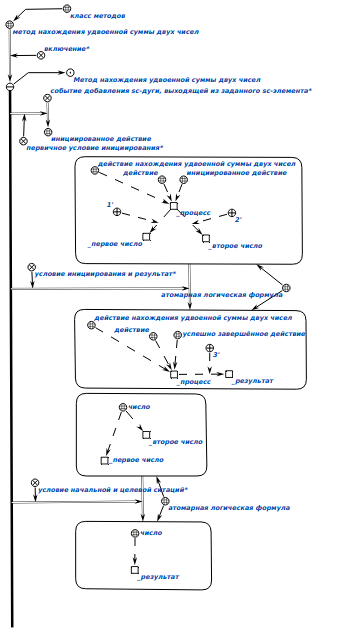
\includegraphics[scale=0.7]{author/part3/figures/condition_and_result.png}
  \caption{Спецификация метода решения задачи вычисления удвоенной суммы двух чисел}
  \label{fig:condition_and_result}
\end{figure}

Программы в зависимости от его способа задания в конкретном языке представления методов будут различаться. В этом можно убедиться, сравнив примеры процедурного (рис. \nameref{fig:procedural_program}) и логического (рис. \nameref{fig:logic_program}) методов решения одной и той же задачи.

\begin{figure}[htbp]  
  \center
  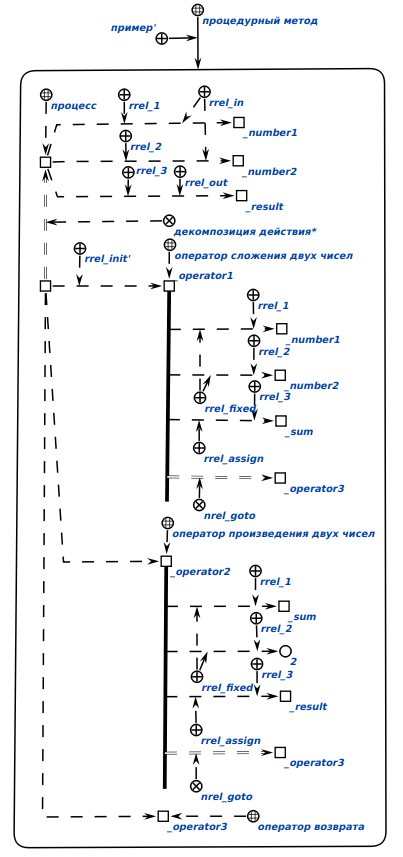
\includegraphics[scale=0.6]{author/part3/figures/procedural_program.png}
  \caption{Пример процедурного метода решения задачи вычисления удвоенной суммы двух чисел}
  \label{fig:procedural_program}
\end{figure}

\begin{figure}[htbp]
  \center
  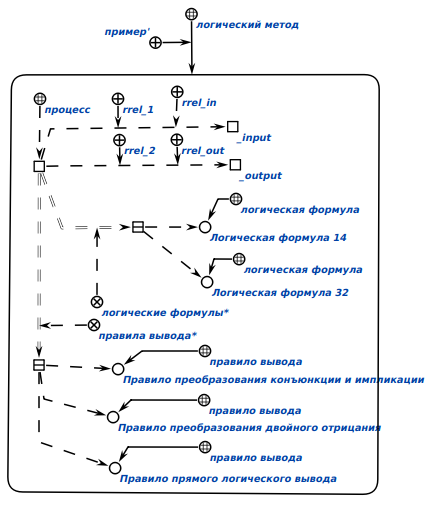
\includegraphics[scale=0.6]{author/part3/figures/logic_program.png}
  \caption{Пример логического метода решения задачи вычисления удвоенной суммы двух чисел}
  \label{fig:logic_program}
\end{figure}

С помощью \textit{SC-кода} можно представлять и те языки, которые не написаны на нём. Проблема будет в том, что форма и смысл языка и его методов будут разделены, то есть будут представлены по-разному. В данном случае \textit{SC-код} выступает мощным инструментом для интеграции спецификаций различных языков внешнего представления знаний. Однако стоит отметить, что в представлении различных форм методов, принадлежащих разным \textit{языкам представления методов}, в рамках \textit{Технологии OSTIS} нет необходимости. Это объясняется тем, что:
\begin{textitemize}
    \item \textit{SC-код} является достаточно универсальным языком для представления любых видов знаний. Это означает, что различные формы алгоритма решения одной и той же задачи можно свести к минимуму. В \textit{SC-коде} фундаментом является формальная теория, что обеспечивает универсальное представление различных видов декларативных и процедурных знаний. Так, логические методы можно представлять в виде процедурных программ, в которых в качестве операндов операторов будут не только логические формулы и \textit{правила вывода}, но и другие методы, обеспечивающее интерпретацию этих \textit{логических формул} при помощи правил вывода. Таким образом, SC-коде можно называть не только языком унифицированного представления знания, но и языком, на котором можно решать различные классы задачи одним и тем же способом.
    \item Различные виды знаний в \textit{ostis-системах}, проектируемые по принципам \textit{Технологии OSTIS} глубоко интегрированы между собой. Это даёт не только простоту для создания этих систем на базе имеющихся языков, которые могут быть описаны на \textit{SC-коде}, но большие возможности для создания базовых \textit{языков программирования} для компьютерных систем нового поколения таких, как, например, \textit{базового языка представления процедурных методов SCP}, \textit{базового языка представления продукционных методов} и так далее. Современные \textit{языки представления методов} создаются с целью упрощения описания какого-то алгоритма для быстрого и качественного решения определённого класса задач \cite{Benri2000}. В свою очередь, предлагаемые методики и модели позволяют проектировать языки представления методов для компьютерных систем нового поколения с помощью базовых \textit{языков представления знаний} таким образом, чтобы сама форма представления знаний не менялась. Методы разных \textit{языки представления методов} должны иметь одну универсальную форму представления, то есть один и тот же синтаксис, но могут давать возможности описывать и представлять разными способами \textit{денотационную} и \textit{операционную семантику} своих \textit{методов} с помощью одного и того же синтаксиса.
    \item Проектирование новых языков представления методов должно сводится к их полному описанию на минимальном семействе \textit{языков SC-кода}: самого \textit{SC-кода}, \textit{SCP} и \textit{SCL}. Речь идёт о том, чтобы спроектировать новый \textit{язык представления методов} достаточно разработать (неатомарный) метаметод на \textit{языках SCP} и \textit{SCL}, который будет интерпретировать методы проектируемых языков, а также описать денотационную семантику этих методов. \textit{Метаметод интерпретации методов языков представления методов} можно называть интерпретатором этих языков, то есть некоторой абстрактной sc-машиной, на которой возможно выполнение методов определённого языка представления этих методов.
\end{textitemize}

\subsection{Операционная семантика программ в ostis-системах}
\label{sec_programs_method_op_semantic}

Полная \textit{спецификация метода*} кроме \textit{денотационной семантики этого метода*} должна включать \textit{операционную семантику этого метода*}, то есть формальное описание интерпретатора заданного метода. \textit{Операционная семантика языка представления методов} описывает выполнение метода, составленного на данном языке, средствами виртуального компьютера. Виртуальный компьютер определяется как абстрактный автомат. Внутренние состояния этого автомата моделируют состояния вычислительного процесса при выполнении метода. Автомат транслирует исходный текст метода в набор формально определенных операций. Этот набор задает переходы автомата из исходного состояния в последовательность промежуточных состояний, изменяя значения переменных метода. Автомат завершает свою работу, переходя в некоторое конечное состояние. Таким образом, здесь идет речь о достаточно прямой абстракции возможного использования языка представления методов. Операционная семантика описывает смысл метода путем выполнения его операторов на простой машине-автомате. Изменения, происходящие в состоянии машины при выполнении данного оператора, определяют смысл этого оператора.

\textit{Операционная семантика} конкретного \textit{метода} сводится к описанию \textit{метаметода}, который его интерпретирует, верифицирует и так далее.

\begin{SCn}
\scnheader{метаметод}
\scnsubset{метод}
\scnidtf{метод, значениями параметров которого являются другие методы}
\end{SCn}

\begin{SCn}
\scnheader{операционная семантика метода}
\scnhaselement{метаметод интерпретации*}
\begin{scnindent}
    \begin{scnreltovector}{декартово произведение}
        \scnitem{класс методов}
        \scnitem{метод}
    \end{scnreltovector}
\end{scnindent}
\scnhaselement{метаметод верификации и оценки качества*}
\begin{scnindent}
    \begin{scnreltovector}{декартово произведение}
        \scnitem{класс методов}
        \scnitem{метод}
    \end{scnreltovector}
\end{scnindent}
\end{SCn}

Отношение \textit{метаметод интерпретации*} представляет собой класс sc-связок между sc-связкой, обозначающей множество методов, и sc-узлом, обозначающим метод, который способен произвести интерпретацию заданного множества методов.
Отношение \textit{метаметод верификации и оценки качества*} представляет собой класс sc-связок между sc-связкой, обозначающей множество методов, и sc-узлом, обозначающим метод, который способен произвести верификацию и оценку качества заданного множества методов.

В рамках \textit{Технологии OSTIS} таких метаметодов может быть большое разнообразие. Каждый из них может состоять из множества атомарных и неатомарных подметодов. Это могут быть как метаметоды, интерпретирующие методы определённых \textit{языков представления методов}, так и метаметоды, верифицируюшие и анализирующие качество этих методов. В том числе метаметоды могут производить операции над другими метаметодами.

\begin{SCn}
\scnheader{метаметод интерпретации методов базовых языков представления методов}
\begin{scnrelfromlist}{класс подметодов}
    \scnitem{метаметод интерпретации методов языка представления логических методов SCP}
    \scnitem{метаметод интерпретации методов языка представления логических методов SCL}
    \scnitem{метаметод интерпретации методов языка представления продукционных методов}
    \scnitem{метаметод интерпретации методов языка представления функциональных методов}
    \scnitem{метаметод интерпретации методов языка представления нейросетей}
    \scnitem{метаметод интерпретации методов языка представления генетических алгоритмов}
\end{scnrelfromlist}
\end{SCn}

\begin{SCn}
\scnheader{метаметод верификации и оценки качества методов базовых языков представления методов}
\begin{scnrelfromlist}{класс подметодов}
    \scnitem{метаметод верификации и оценки качества методов языка представления логических методов SCP}
    \scnitem{метаметод верификации и оценки качества методов языка представления логических методов SCL}
    \scnitem{метаметод верификации и оценки качества методов языка представления продукционных методов}
    \scnitem{метаметод верификации и оценки качества методов языка представления функциональных методов}
    \scnitem{метаметод верификации и оценки качества методов языка представления нейросетей}
    \scnitem{метаметод верификации и оценки качества методов языка представления генетических алгоритмов}
\end{scnrelfromlist}
\end{SCn}

Так, например, при реализации методов в оstis-системах метаметодами будут являться \textit{интепретатор базового языка программирования SCP}, а также интепретаторы, реализованные непосредственно на \textit{языке SCP}. 

Понятие синтакиса, денотационной и операционной семантики языков представления методов сводятся к понятию синтаксиса, денотационной и операционной семантики вообще любого языка.

\section{Синтаксис и семантика языков программирования в ostis-системах}
\label{sec_programs_method_representation_language_syntax_and_semantic}

Понятно, что для использования \textit{языка представления методов} следует описать каждую конструкцию языка в отдельности, а также ее применение в совокупности с другими конструкциями. В языке существует множество различных конструкций, точное определение которых необходимо как программисту, применяющему язык, так и разработчику компилятора для этого языка. Программисту эти знания позволяют прогнозировать вычисления, производимые операторами метода. Разработчику описания конструкций необходимы для создания правильной реализации компилятора.

Описание формальной модели \textit{языка программирования} можно задать его \textit{спецификацией}. Спецификация содержит описание \textit{синтаксиса} и \textit{семантики языка представления методов}.

\begin{SCn}
\scnheader{спецификация языка представления методов*}
\scnsuperset{отношение, заданное на множестве (язык представления методов)*}
\begin{scnrelfromset}{разбиение}
    \scnitem{синтаксис языка представления методов*}
    \begin{scnindent}
        \scnsubset{синтаксис языка*}
        \scnidtf{быть теорией правильно построенных информационных конструкций, принадлежащих заданному языку представления методов}
    \end{scnindent}
    \scnitem{денотационная семантика языка представления методов*}
    \begin{scnindent}
        \scnsubset{денотационная семантика языка*}
        \scnidtf{обобщенная формулировка классов задач, решаемых с помощью данного языка представления методов*}
    \end{scnindent}
    \scnitem{операционная семантика языка представления методов*}
    \begin{scnindent}
        \scnsubset{операционная семантика языка*}
        \scnidtf{перечень обобщенных агентов, обеспечивающих интерпретацию методов заданного языка представления методов*}
        \scnidtf{семейство методов интерпретации текстов данного языка представления методов*}
        \scnidtf{формальное описание интерпретатора заданного языка представления методов*}
    \end{scnindent}
\end{scnrelfromset}
\end{SCn}

Под \textit{синтаксисом языка представления методов*} подразумевается бинарное ориентированное отношение, каждая пара которого связывает знак некоторого языка с описанием синтаксически выделяемых классов фрагментов конструкций заданного языка представления методов, с описанием отношений, заданных на этих классах и с конъюнкцией кванторных высказываний, являющихся синтаксическими правилами заданного языка, то есть правилами, которым должны удовлетворять все синтаксические правильные (правильно построенные) конструкции указанного языка представления методов В общем случае, отношение \textit{синтаксиса языка представления методов*} ничем не отличается от отношения \textit{синтаксиса языка*}, но всё-таки уточнение есть, поскольку языка представления методов являются языками вообще и синтаксис языка представления методов наследует все свойства синтаксиса любых языков. \textit{Синтаксиса языка представления методов*} объединяет синтаксисы всех методов, принадлежащих данному языку представления методов.

Под \textit{денотационной семантикой языка представления методов*} подразумевается бинарное ориентированное отношение, каждая пара которого связывает знак некоторого языка со знаком некоторой онтологии, с помощью которой можно описывать методы этого языка, а под \textit{операционной семантикой языка представления методов*} -- описание метаметода интерпретации методов этого языка.

\section{Система поддержки проектирования и разработки программ в ostis-системах}
\label{sec_programs_help_system}

Текущее состояние в области проектирования и разработки программного обеспечения говорит о том, что разработчики больше стремятся автоматизировать разработку методов на конкретных языках представления методов, чем обеспечить инструментальными обучающими средствами их проектирования, в том числе проектирования новых языков представления методов. Это приводит к следующим проблемам:
\begin{textitemize}
	\item В то время, как количество разработчиков, понимающих код какой-то сложной программной системы, уменьшается, требования к этой системе растут всё быстрее и быстрее. Зачастую, разработчики сложных программных систем сами не в состоянии объяснить логику работы этих систем. По этой причине необходимо создавать инструментальные средства, которые будут позволять автоматизировать документирование программных систем \cite{lu2022rethinking}.
	\item Для обучения новых разработчиков навыкам работы с программными системы и их разработки необходимо привлекать ресурсы экспертов, понимающих принципы работы этих программных систем. Проблема решается разработкой справочной системы, которая будет позволять не только обучать пользователя тому, как проектировать методы решения задачи и программные системы на основе этих методов, но и указывать на пробелы в смежных дисциплинах, необходимых для достижения качественных результатов всей своей деятельности.
	\item В инженерии часто разработчики проектируют и разрабатывают решения, которые уже когда-то были созданные другими специалистами. Таким образом, получаются функционально эквивалентные методы решения задач, а то, и вовсе, программные системы, решающие схожие проблемы. Ключом к решению данной проблемы является проектирование семантически мощной библиотеки многократно используемых методов решения задач.
\end{textitemize}

Таким образом, одной семантической теории программ недостаточно. Кроме неё, для перманетного и беспрепятственного проектирования и разработки методов различного класса необходимо разрабатывать:
\begin{textitemize}
	\item интеллектуальную систему поддержки проектирования и разработки методов, упомянутую в работе \cite{Gulakina2012}, которая будет не только помогать разработчику верифицировать разрабатываемый метод, но и подсказывать способы его разработки;
	\item семантически мощную библиотеку многократно используемых компонентов \cite{Ford2019} для быстрого поиска существующих методов решения задач и их применения для решения других более комплексных задач \cite{sales2022explainable}.
\end{textitemize}

Потенциальная система должная быть частью общего инструментального средства разработки интеллектуальны компьютерных систем нового поколения - ostis-платформы \cite{Platform2021} - и может состоять из следующих компонентов:
\begin{textitemize}
	\item интеллектуальной help-системы по семантической теории программ;
	\item интеллектуальной help-системы по библиотеке многократно используемых методов решения задач,
	\item интеллектуальной help-системы по комплексу инструментальных средств проектирования  методов решения задач,
	\item интеллектуальной help-системы по методике обучения проектированию различных методов решения задач.
\end{textitemize}

Каждый компонент должен содержать:
\begin{textitemize}
	\item справочную подсистему,
	\item подсистему мониторинга и анализа деятельности разработчика методов решения задач,
	\item подсистему управления обучением.
\end{textitemize}

Каждая из подсистем взаимодействует с другими подсистемами, а также может функционировать автономно.

Справочная подсистема является консультантом-экспертом в области семантической теории программ, который может ответить на любой вопрос новичка или опытного пользователя. Каждая из таких систем может становится индивидуальным помощников в обучении новых специалистов - персональным ostis-ассистентом.

\section{Свойства, определяющие эффективность программ в ostis-системах}
\label{sec_programs_method_kriteria}

\textit{Язык представления методов} можно определить множеством показателей, характеризующих отдельные его свойства. Возникает задача введения меры для оценки степени приспособленности языка представления методов к выполнению возложенных на него функций — \textit{критерии эффективности} \cite{Orlov2013}. Критерии эффективности методов приводятся на основе частных показателей эффективности этих методов (показателей качества). Способ связи между частными показателями определяет вид критерия эффективности.

\begin{SCn}
\scnheader{эффективность метода}
\begin{scnrelfromlist}{свойство-предпосылка}
    \scnitem{легкость чтения и понимания метода}
    \scnitem{легкость представления метода}
    \scnitem{стоимость метода}
    \scnitem{общий объем задач, решаемых при помощи данного класса методов}
    \scnitem{многообразие видов задач, решаемых при помощи данного класса методов}
    \scnitem{надёжность метода}
\end{scnrelfromlist}
\end{SCn}

\textit{Лёгкость чтения метода} должна способствовать легкому выделению основных понятий каждой части метода без обращения к его спецификации.

\begin{SCn}
\scnheader{легкость чтения и понимания метода}
\begin{scnrelfromlist}{свойство-предпосылка}
    \scnitem{простота синтаксиса языка представления методов}
    \scnitem{ортогональность информационных конструкций языка представления методов}
    \scnitem{структурированность потока управления в методе}
\end{scnrelfromlist}
\end{SCn}

\textit{Язык представления методов} должен предоставить \textit{простой} набор \textit{информационных конструкций}, которые могут быть использованы в качестве базисных элементов при создании методов.
Сильное воздействие на простоту оказывает \textit{синтаксис языка}: он должен прозрачно отражать семантику конструкций, исключать двусмысленность и неоднозначность толкования.

\textit{Ортогональность} означает, что любые возможные комбинации различных информационных конструкций будут осмысленными, без неожиданного поведения, возникающих в результате взаимодействия конструкций или контекста использования.

Порядок передач управления между операторами метода, то есть \textit{поток управления}, должен быть удобен для чтения и понимания человеком.

\textit{Легкость создания метода} отражает удобство языка для представления этого метода в конкретной предметной области.

\begin{SCn}
\scnheader{легкость представления метода}
\begin{scnrelfromlist}{свойство-предпосылка}
    \scnitem{простота синтаксиса языка представления методов}
    \scnitem{естественность синтаксиса языка представления методов}
    \scnitem{ортогональность информационных конструкций языка представления методов}
    \scnitem{полнота и точность спецификации языка представления методов}
    \scnitem{согласованность и целостность спецификации языка представления методов}
\end{scnrelfromlist}
\end{SCn}

\textit{Синтаксис метода} должен способствовать легкому и прозрачному отображению в нем алгоритмических структур предметной области. \textit{Синтаксис языка представления методов} должен быть не только \textit{простым}, но и \textit{естественным}, и поддерживать \textit{ортогональность} информационных конструкций языка.

\textit{Лёгкость представления нового метода} обеспечивается \textit{полной и точной, согласованной и целостной спецификацией} соответствующего языка. То есть необходимо достаточное количество \textit{информационных конструкций} в этом языке для того чтобы представить конкретный \textit{метод}. При этом \textit{спецификация языка} должна быть согласованной и целостной чтобы представлять на ней непротиворечивые \textit{методы}.

\textit{Стоимость метода языка представления методов} складывается из нескольких составляющих:

\begin{SCn}
\scnheader{общая стоимость метода}
\begin{scnrelfromlist}{свойство-предпосылка}
    \scnitem{стоимость применения метода}
    \scnitem{стоимость интерпретации метода}
    \scnitem{стоимость создания, тестирования и использования метода}
    \scnitem{стоимость сопровождения метода}
    \scnitem{согласованность и целостность спецификации языка представления методов}
\end{scnrelfromlist}
\end{SCn}

\textit{Стоимость применения метода} во многом зависит от структуры \textit{языка представления методов}. Язык, требующий многочисленных проверок синтаксических типов во время применения метода, будет препятствовать быстрой работе программы.

\textit{Размер стоимости интерпретации метода} зависит от возможностей используемого метаметода интерпретации. Чем совершеннее методы оптимизации, тем дороже стоит интерпретация.
Размер стоимости создания, тестирования и использования метода зависит от используемого метаметода верификации и оценки качества этого метода.

Многочисленные исследования показывают, что значительную часть стоимости используемого метода составляет не стоимость его разработки, а \textit{стоимость его сопровождения} \cite{Brooks2021}. Связывая сопровождение методов с другими их характеристиками, следует выделить, прежде всего, зависимость от читабельности, поскольку сопровождение обычно происходит следующим поколением разработчиков.

\textit{Общий объем задач и многообразие видов задач, решаемых при помощи данного класса методов}, являются не менее важными характеристиками и показывают степень универсальности соответствующего языка представления методов. Чем больше задач можно решить на я.п.м, тем больше он универсальнее.

\textit{Надёжность методов языка представления методов} должно обеспечиваться минимумом ошибок при работе конкретного метода.

Все эти критерии можно применить и касательно самих языков представления методов.

\section*{Заключение к Главе \ref{chapter_programs}}

Данная глава является началом \textit{Семантической теории программ для компьютерных систем нового поколения}. Логичным развитием данной главы будут:

\begin{textitemize}
    \item уточнение и дополнение понятий \textit{Предметной области и онтологии методов} для достижения полноты теории;
    \item описание дочерних предметных областей \textit{Предметной области и онтологии методов} для конкретных видов методов, а также уточнение денотационной и операционной семантики спецификации этих методов;
    \item описание возможных путей реализации метаметодов интерпретации методов различных я.п.м;
    \item формализация математических моделей для подсчёт оценок эффективности методов.
\end{textitemize}
